\documentclass[11pt,a4paper]{article}
\usepackage[margin=2.5cm,top=2.6cm,bottom=2.4cm]{geometry}
\usepackage{fontspec}
\setmainfont{Bitstream Charter}
\setsansfont{Inter}[Scale=0.95]
\setmonofont{DejaVu Sans Mono}[Scale=0.82]
\usepackage{microtype,xcolor,graphicx,booktabs,array,enumitem,caption,float,fancyhdr,titlesec,hyperref,tikz}\usepackage[skins]{tcolorbox}
\usetikzlibrary{positioning,arrows.meta,shapes.geometric,calc}
\definecolor{ink}{HTML}{17202B}\definecolor{blue}{HTML}{1F6FEB}\definecolor{teal}{HTML}{0F9D8A}\definecolor{amber}{HTML}{D98E04}\definecolor{red}{HTML}{D1344B}\definecolor{mute}{HTML}{6B7785}\definecolor{paper}{HTML}{F3F5F8}
\hypersetup{colorlinks=true,linkcolor=blue,urlcolor=blue,citecolor=blue,pdftitle={Field Data Quality Lab},pdfauthor={Samatar Ahmed}}
\color{ink}
\titleformat{\section}{\sffamily\bfseries\Large\color{ink}}{\thesection}{0.7em}{}
\titleformat{\subsection}{\sffamily\bfseries\large\color{ink}}{\thesubsection}{0.7em}{}
\titleformat{\subsubsection}{\sffamily\bfseries\normalsize\color{ink}}{}{0em}{}
\titlespacing*{\section}{0pt}{2.2ex}{1.2ex}\titlespacing*{\subsection}{0pt}{1.8ex}{0.8ex}
\captionsetup{font={small,sf},labelfont={bf},labelsep=period,justification=raggedright,singlelinecheck=false,skip=6pt}
\setlength{\parskip}{0.55em}\setlength{\parindent}{0pt}\linespread{1.07}
\pagestyle{fancy}\fancyhf{}\renewcommand{\headrulewidth}{0.3pt}
\fancyhead[L]{\sffamily\small\color{mute}Field Data Quality Lab}\fancyhead[R]{\sffamily\small\color{mute}Samatar Ahmed}\fancyfoot[C]{\sffamily\small\color{mute}\thepage}
\setlist{itemsep=2pt,topsep=3pt,leftmargin=1.4em}
\newtcolorbox{callout}[1][]{colback=paper,colframe=paper,boxrule=0pt,left=10pt,right=10pt,top=7pt,bottom=7pt,borderline west={2.5pt}{0pt}{blue},sharp corners,fontupper=\small,#1}
\newtcolorbox{warn}{colback=paper,colframe=paper,boxrule=0pt,left=10pt,right=10pt,top=7pt,bottom=7pt,borderline west={2.5pt}{0pt}{amber},sharp corners,fontupper=\small}
\newcommand{\simd}{\textcolor{amber}{\sffamily\bfseries simulated}}
\newcommand{\real}{\textcolor{teal}{\sffamily\bfseries real data}}
\begin{document}
\thispagestyle{empty}
\begin{tikzpicture}[remember picture,overlay]
 \fill[ink] (current page.north west) rectangle ([yshift=-9.2cm]current page.north east);
 \fill[blue] ([yshift=-9.2cm]current page.north west) rectangle ([yshift=-9.35cm,xshift=7cm]current page.north west);
\end{tikzpicture}
\vspace*{1.2cm}
{\color{white}\sffamily
{\Huge\bfseries Field Data Quality Lab\par}\vspace{0.6em}
{\Large From raw phone-survey data to a defensible causal estimate:\\[2pt] automated quality checks, a simulation stress test, and\\[2pt] a randomised evaluation of SMS farm advice in Kenya\par}}
\vspace{5.6cm}
{\sffamily\large Samatar Ahmed\par}
{\sffamily\color{mute} November 2026\par}
\vspace{1.2em}
\begin{minipage}{0.82\textwidth}\small
Data: Fabregas, Kremer, Lowes, On \& Zane (2024), \emph{Digital Information Provision and Behavior Change: Lessons from Six Experiments in East Africa}, openICPSR project 186241. Survey estimates in this report use only the two Precision Agriculture for Development (now Precision Development) trials, PAD1 and PAD2. Call times, durations and planted problems are \textbf{simulated} and labelled throughout. Code, do-files, instrument and interactive dashboard accompany this report.
\end{minipage}
\clearpage
\tableofcontents
\clearpage

\section*{Executive summary}
\addcontentsline{toc}{section}{Executive summary}
\textbf{The question.} A research team collects thousands of phone interviews through dozens of field officers. How quickly can it find an officer whose data cannot be trusted, how often will it be wrong when it tries, and does any of it change the estimate of what the programme did?

\textbf{What I built.} A complete, reproducible pipeline on two real randomised trials of SMS agronomic advice in western Kenya: a validated build of the analysis panels (19/19 integrity checks passed), a high-frequency check (HFC) engine that scores every field officer, a SurveyCTO-ready instrument with the controls built in, a simulation that plants known problems and measures detection power, an experimental analysis with multiple-testing control, and a dashboard. The package spans 38 files and 756\,586 rows; the generic QA suite handles the largest file ($202\,972\times35$) in 0.41 seconds.

\begin{callout}
\textbf{Five findings}
\begin{enumerate}
\item \textbf{Field-officer differences are real, not noise.} In PAD2, 13 of 26 officers are flagged (4 red, 9 amber). Shuffling officer labels, the same rule flags 0.21 officers on average. In PAD1, 1 red and 3 amber.
\item \textbf{Flags rest on process, not on outcomes.} The instrument enforces skip logic (zero violations in both trials), so the signal comes from path length, skip-trigger answers and a deficit of ``don't know'' answers. All four red PAD2 officers show both a shortcut pattern and a don't-know deficit.
\item \textbf{Simple rules misfire; calibrated rules do not.} A significance-only speed test flags 30\% of honest officers because honest officers differ in pace. Adding a 20\% effect-size floor and false-discovery control cuts that to 0.5\%; requiring corroboration cuts it to 0.0\%.
\item \textbf{A 40\%-shorter enumerator is caught within about 23 interviews} in simulation (power 99\%). The don't-know deficit is a weak detector at the real base rate (0.75\%): corroborated power falls to 88\%. Timing and a back-check carry the load.
\item \textbf{The programme result survives every quality filter.} Any SMS raised reported lime use by 4.9 percentage points (control 18\%). The estimate is 5.0 with officer fixed effects, 5.1 after dropping red officers. Coupon records show a smaller rise (1.7 points, not significant), so the survey figure should be read as an upper bound.
\end{enumerate}
\end{callout}

\textbf{What this is not.} A flag is a prompt to back-check, never evidence of misconduct. The raw surveys carry no timestamps, so all paradata are simulated and labelled. The Stata do-files were written but not executed in the build environment, and the XLSForm was validated structurally rather than compiled by an official engine (Section~\ref{sec:limits}).

\section{Why data quality deserves its own project}
Impact evaluations are only as good as the interviews behind them. Three failure modes recur in phone and face-to-face surveys. \emph{Shortcutting}: an enumerator answers gate questions so that follow-up modules are skipped. \emph{Fabrication}: interviews are invented, often by copying earlier answers. \emph{Drift}: pace and care change over a long field period. All three leave traces in the data long before anyone looks, if the team looks systematically and daily.

The practical difficulty is not computing a statistic. It is deciding \emph{when a pattern is a signal}. Officers legitimately differ in pace, language and the respondents they reach. A rule that flags every deviation floods supervisors with false alarms and teaches them to ignore the system. A rule that is too strict finds problems after the survey ends. This report treats that calibration as the central problem, and answers it with data: real interviews to learn what normal variation looks like, simulated problems to learn what the rules can and cannot catch.

\subsection*{How to read this report}
Every figure and table carries a source tag. \real{} marks estimates from the PAD1/PAD2 survey files. \simd{} marks anything involving call times, durations or planted problems. Sections~\ref{sec:data}--\ref{sec:system} describe the data and the system, Section~\ref{sec:audit} audits the real data, Section~\ref{sec:sim} stress-tests the rules, Sections~\ref{sec:impact}--\ref{sec:robust} estimate programme effects and test whether quality changes them, and Section~\ref{sec:recs} turns the lessons into an operating procedure.

\section{Data and trial design}\label{sec:data}
\subsection{The two trials}
Precision Agriculture for Development (PAD, now Precision Development) sends free SMS agronomic advice to smallholder maize farmers in western Kenya. PAD1 and PAD2 tested personalised advice on lime and fertiliser. Farmers were randomised individually; endline interviews were conducted by phone by field officers (FOs).

\begin{table}[H]\centering\small\setlength{\tabcolsep}{6pt}
\begin{tabular}{lrr}\toprule & PAD2 (primary) & PAD1 (replication)\\\midrule
Farmers at baseline & 5\,890 & 1\,897\\ Endline interviews & 4\,933 & 1\,511\\ Field officers & 26 & 23\\
Arms & Control, SMS, SMS+Call offer, SMS+Call & Control, General SMS, Local SMS\\
Response rate, control / treated & 84.1\% / 83.6\% & 79.4\% / 79.4\%\\\bottomrule\end{tabular}
\caption{The two trials analysed. \real}\end{table}

\subsection{The wider package, and what ``large'' means here}
The openICPSR package contains six experiments. Its raw files total 756\,586 rows in 38 files (about 10.4 million non-missing cells). I used it to check that the QA logic scales: the generic suite (missingness, duplicate keys, constant columns, extreme outliers) reads and checks the largest file in under a second.
\begin{table}[H]\centering\small\setlength{\tabcolsep}{6pt}\begin{tabular}{llrr}
\toprule
Study & File & Rows & Columns \\
\midrule
OAF3 & OAF3\_admin\_sample\_raw.csv & 202\,972 & 35 \\
OAF3 & OAF3\_treat\_LR2019\_raw.csv & 194\,336 & 3 \\
OAF3 & OAF3\_admin\_LR2018\_raw.csv & 125\,811 & 6 \\
OAF3 & OAF3\_admin\_LR2019\_raw.csv & 91\,672 & 4 \\
OAF2 & OAF2\_baseline\_LR2017\_raw.csv & 32\,572 & 30 \\
OAF2 & OAF2\_clients\_LR2018\_raw.csv & 24\,825 & 10 \\
OAF2 & OAF2\_clients\_LR2019\_raw.csv & 18\,356 & 2 \\
Other & soil\_test.csv & 9\,213 & 7 \\
\bottomrule
\end{tabular}\caption{Largest raw files in the package. \real}\end{table}

\subsection{Outcomes}
Survey outcomes (observed for respondents): heard of lime; names lime as a remedy for soil acidity; used lime in the long rains of 2017; used urea. Administrative outcomes (observed for \emph{every} farmer): redeemed a lime coupon; redeemed a fertiliser coupon. Administrative outcomes are immune to survey attrition and to anything an enumerator does, which is why they appear alongside the survey measures throughout.

\subsection{Arm labels: a documentation problem}
In the replication code the raw labels \texttt{t1} and \texttt{t3} are relabelled with a comment ``fix order'', and the variable labels say raw \texttt{t1} is SMS+Call and raw \texttt{t3} is SMS. A later string variable assigns them the other way round. I could not resolve this from the data. The primary contrast therefore \emph{pools all SMS arms against control}, which does not depend on the mapping; arm-level estimates are secondary and flagged.

\section{The quality-assurance system}\label{sec:system}
\begin{figure}[H]\centering
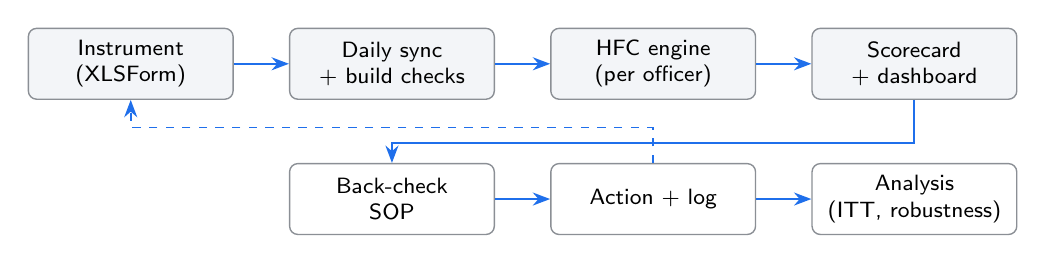
\begin{tikzpicture}[node distance=7mm,font=\sffamily\footnotesize,box/.style={draw=ink!50,rounded corners=3pt,fill=paper,minimum height=9mm,minimum width=26mm,align=center,line width=0.5pt},arr/.style={-{Stealth[length=2.2mm]},line width=0.7pt,color=blue}]
\node[box] (a) {Instrument\\(XLSForm)};\node[box,right=of a] (b) {Daily sync\\+ build checks};\node[box,right=of b] (c) {HFC engine\\(per officer)};\node[box,right=of c] (d) {Scorecard\\+ dashboard};
\node[box,below=8mm of b,fill=white] (e) {Back-check\\SOP};\node[box,right=of e,fill=white] (f) {Action + log};\node[box,right=of f,fill=white] (g) {Analysis\\(ITT, robustness)};
\draw[arr](a)--(b);\draw[arr](b)--(c);\draw[arr](c)--(d);\draw[arr](d)--++(0,-1.0)-|(e);\draw[arr](e)--(f);\draw[arr](f)--(g);\draw[arr,dashed](f.north)--++(0,0.45)-|(a.south);
\end{tikzpicture}
\caption{The pipeline. The dashed line closes the loop: findings change the instrument and the checks.}\end{figure}

\subsection{Quality is designed into the instrument}
The accompanying XLSForm (\texttt{xlsform/pxd\_lime\_midline\_LR2017.xlsx}, 80 rows, 73 fields) is based on the public PAD2 questionnaire. Controls include: double entry of the farmer ID with a hard match constraint; pre-loaded respondent checks; skip logic mirroring the paper form; hard constraints with messages (planted acres cannot exceed total land; lime area cannot exceed planted area); a single consistent code for ``don't know'' ($-99$ for numbers, 99 for categories) with propagation so a don't-know on land size does not block later constraints; mutually exclusive multi-select answers; a soft warning for implausible lime rates; and built-in paradata (a text audit, total duration, section timers, and calculate fields for don't-know count, gate-``No'' count and a too-fast flag). The settings sheet carries a slot for the encryption public key. A test plan of 21 cases is provided. Structural validation: 11/11 checks pass.

\subsection{The HFC rules}
Appendix~\ref{app:hfc} lists every rule. Three design choices matter.
\begin{itemize}
\item \textbf{Adjust before comparing.} Each metric is residualised on treatment arm, baseline covariates and location fixed effects. Officers are compared on what is left.
\item \textbf{Permute, don't assume.} Officer labels are shuffled \emph{within location} 4,000 times to build the null for each officer and metric. This is valid for rare events such as don't-know answers, where normal approximations fail. Benjamini--Hochberg q-values control false discoveries across officers.
\item \textbf{Count behaviours, not metrics.} Path length and skip-trigger answers are mechanically linked ($r=-0.62$), so they form one family. An officer is red if two independent families reach red level or three are flagged.
\end{itemize}

\subsection{Mirror implementations and data protection}
The engine exists in Python (executed, source of every number here) and as a Stata do-file suite for teams that work in Stata. The Stata files are \textbf{unexecuted} here; a comparison do-file asserts they reproduce the Python ITT table. Appendix~\ref{app:dp} summarises the data-protection protocol (classification, encryption at source, separation of identifiers, access control, de-identification, retention, incident response).

\section{Auditing the real data}\label{sec:audit}
\subsection{Build and integrity checks}
\real{} The panel builder asserts keys, merges and sample sizes. All 19/19 checks pass: respondent IDs are unique in every file, the randomisation file covers the baseline sample, every endline respondent exists at baseline, all arms map, the treated share is 75\% and every responder has an officer ID.

\subsection{Skip logic is enforced}
Seven consistency rules were applied to the endline (for example, ``never heard of lime'' but ``applied lime''; ``no fertiliser'' but a fertiliser type recorded). Each rule had a large population at risk, from 111 to 4,822 interviews. \textbf{There were no violations in PAD2 or PAD1.} For a CATI instrument this is the expected result of programmed skip logic. It also shows why violations cannot be the signal here; any problem must leave subtler traces.

\subsection{Don't-know answers, straight-lining and duplicates}
The mean don't-know share of categorical answers is only 0.75\% in PAD2 (1.6\% in PAD1), and straight-lining on yes/no items occurs in 1.1\% of PAD2 interviews. At those base rates, single interviews carry almost no information; only patterns over many interviews do.

The duplicate-answer check illustrates why every rule needs an informativeness gate. In PAD2, 53\% of interviews with at least ten answers duplicate another interview's full answer vector, because a short, mostly binary questionnaire has few distinct patterns. The check is therefore \emph{disabled} for PAD2. In PAD1, where quantities are recorded, only 0.4\% duplicate and the check is informative.

\subsection{Field-officer scorecard}
\begin{figure}[H]\centering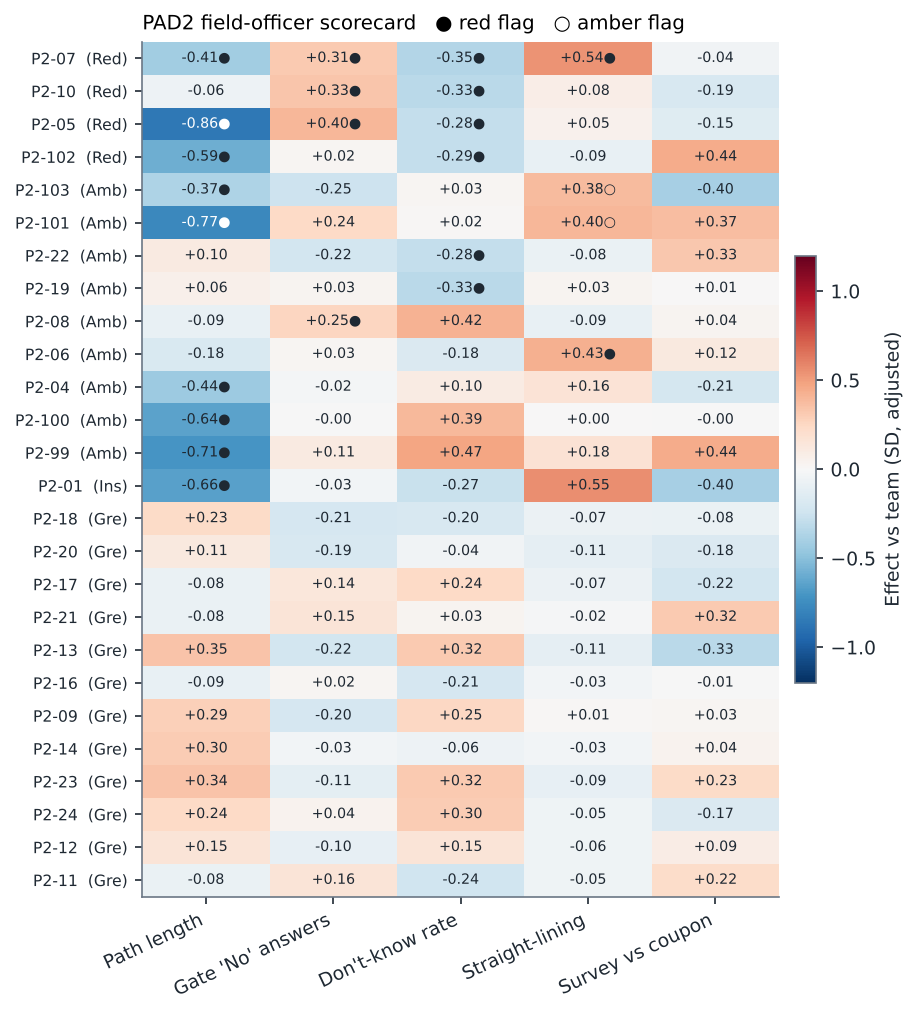
\includegraphics[width=0.78\textwidth]{figures/fig01_fo_heatmap.png}\caption{PAD2 field-officer scorecard. Cells show the difference from the team in standard deviations after adjustment; filled circles mark red flags, open circles amber. \real}\label{fig:heat}\end{figure}

Figure~\ref{fig:heat} and Table~\ref{tab:fo} show the result. Four officers are red, 9 amber, 12 green and 1 has too few interviews to judge. Every red officer pairs a shortcut-family flag (shorter paths or more skip-trigger answers) with a don't-know deficit; one also straight-lines. Omnibus permutation tests reject equal officers for path length, skip triggers, don't-know rate and straight-lining ($p<0.001$ each), but not for survey-versus-coupon discordance ($p=0.44$).
\begin{table}[H]\centering\small\setlength{\tabcolsep}{4pt}\begin{tabular}{lrlrrrl}
\toprule
Officer & Interviews & Tier & Items/interview & DK share (\%) & Straight-line (\%) & Families flagged \\
\midrule
P2-07 & 89 & Red & 12.7 & 0.00 & 6.7 & dk, shortcut, straightline \\
P2-05 & 109 & Red & 11.7 & 0.08 & 1.8 & dk, shortcut \\
P2-10 & 220 & Red & 13.4 & 0.00 & 1.8 & dk, shortcut \\
P2-102 & 66 & Red & 12.3 & 0.13 & 0.0 & dk, shortcut \\
P2-101 & 72 & Amber & 11.9 & 0.80 & 5.6 & shortcut, straightline \\
P2-103 & 78 & Amber & 12.9 & 0.71 & 5.1 & shortcut, straightline \\
P2-04 & 107 & Amber & 12.7 & 0.97 & 2.8 & shortcut \\
P2-06 & 120 & Amber & 13.1 & 0.29 & 5.8 & straightline \\
P2-08 & 264 & Amber & 13.4 & 1.70 & 0.4 & shortcut \\
P2-100 & 73 & Amber & 12.2 & 1.70 & 1.4 & shortcut \\
P2-19 & 313 & Amber & 13.7 & 0.02 & 1.3 & dk \\
P2-22 & 351 & Amber & 13.7 & 0.07 & 0.3 & dk \\
P2-99 & 66 & Amber & 12.1 & 1.81 & 3.0 & shortcut \\
\bottomrule
\end{tabular}\caption{Flagged PAD2 officers. ``Families'' lists the behaviour families flagged. \real}\label{tab:fo}\end{table}

\subsection{Is that more than chance?}
\begin{figure}[H]\centering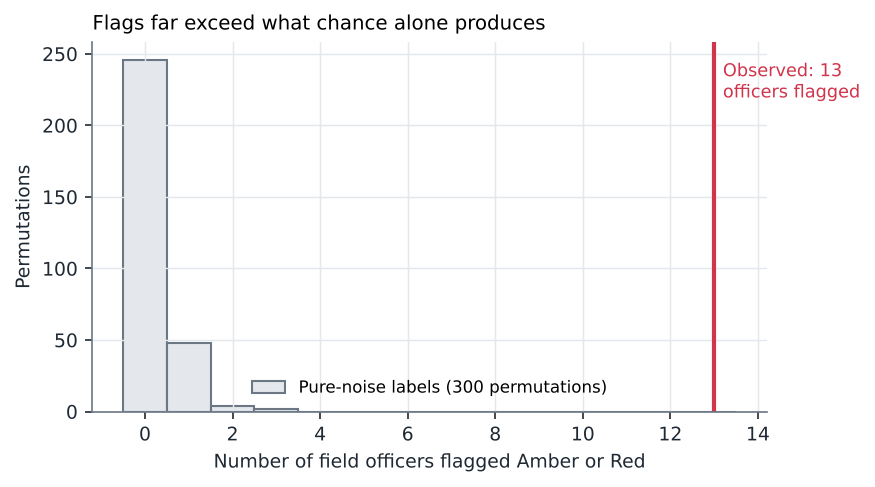
\includegraphics[width=0.62\textwidth]{figures/fig02_null_calibration.png}\caption{Number of officers flagged when officer labels are shuffled (grey), against the number flagged in the real data (red line). \real}\label{fig:null}\end{figure}
To check, the whole tiering rule was run on 300 datasets with officer labels shuffled. It flagged 0.21 officers on average and flagged anyone in only 18\% of shuffles; it \emph{never} produced a red officer. Against that, 13 of 26 real officers are flagged. In PAD1 the null is 0.32 flagged on average (25\% of shuffles flag anyone) against 1 red and 3 amber.

\subsection{What the flags can and cannot mean}
\begin{warn}
Path length depends on respondents' own answers: someone who has heard of lime is asked more questions. If officers are matched to respondents on something unobserved, officers can differ without any misbehaviour. Adjustment for arm, covariates and location removes what I can see. The flags justify a back-check, not a conclusion. The next section asks what the rules can detect when the truth is known.
\end{warn}

\section{Stress-testing the checks with simulated paradata}\label{sec:sim}
\subsection{Design}
The surveys carry no timestamps, so durations, call times and answer signatures here are \simd{}. Only the \emph{workload per officer} mirrors the real data (26 officers, 15 to 351 interviews). Interview length follows the real path-length distribution, plus officer pace and noise. Five officers carry a planted problem; the rest are honest.
\begin{table}[H]\centering\small\setlength{\tabcolsep}{4pt}\begin{tabular}{lllll}
\toprule
Officer & Problem & Planted behaviour & First flagged & First Red \\
\midrule
SIM-03 & Shortcutter & 40\% shorter, 70\% fewer DK & day 4 & day 4 \\
SIM-08 & Fabricator & 12\% copy-paste, 2--4 min bursts & day 3 & day 3 \\
SIM-14 & Off-hours caller & 30\% of calls outside 07:00--20:00 & day 5 & day 5 \\
SIM-19 & Drifter & up to 35\% faster over time & day 15 & day 22 \\
SIM-22 & Fast but honest & 25\% faster, otherwise normal & day 3 & never \\
\bottomrule
\end{tabular}\caption{Planted problems and the day each is first flagged by the daily monitor. \simd}\label{tab:sim}\end{table}

\subsection{What the daily monitor finds}
\begin{figure}[H]\centering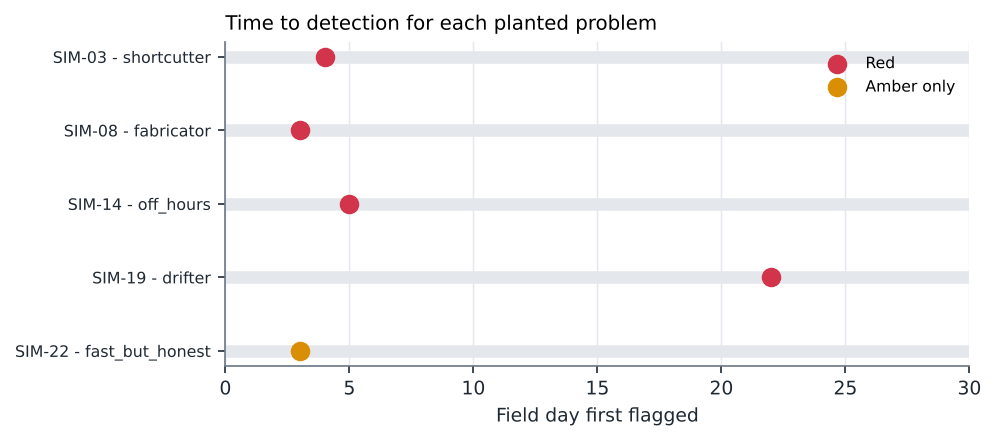
\includegraphics[width=0.78\textwidth]{figures/fig11_detection_timeline.png}\caption{First day each planted officer is flagged (red = escalated to Red, amber = flagged only). \simd}\end{figure}
The shortcutter is escalated on day 4, the fabricator on day 3 and the off-hours caller on day 5. The drifter is flagged amber on day 15 and escalated on day 22, as the decline accumulates. The fast-but-honest officer is flagged on day 3 but is \emph{never escalated}: the speed rule fires, nothing corroborates it, and the tier stays amber. That is the intended behaviour. A fast officer deserves a look, not a suspension. Across all 28 daily checks, none of the 21 honest officers was flagged at the end of the field period.

\begin{figure}[H]\centering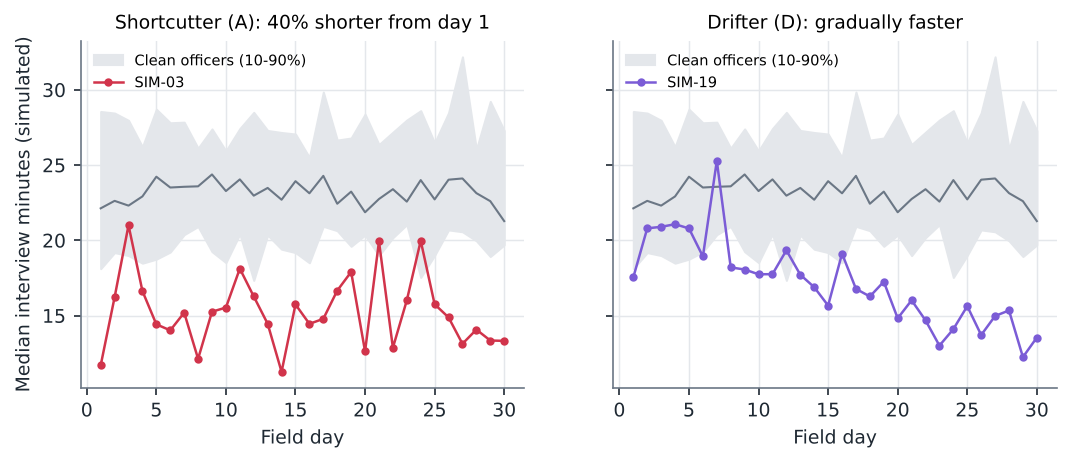
\includegraphics[width=0.86\textwidth]{figures/fig05_sim_durations.png}\caption{Median daily interview length for two planted officers against the band of honest officers. \simd}\end{figure}

\subsection{Power and false alarms}
A Monte Carlo experiment (150 simulated field periods per setting) places one shortcutter among 26 officers and varies how much shorter the interviews are and the baseline don't-know rate.
\begin{figure}[H]\centering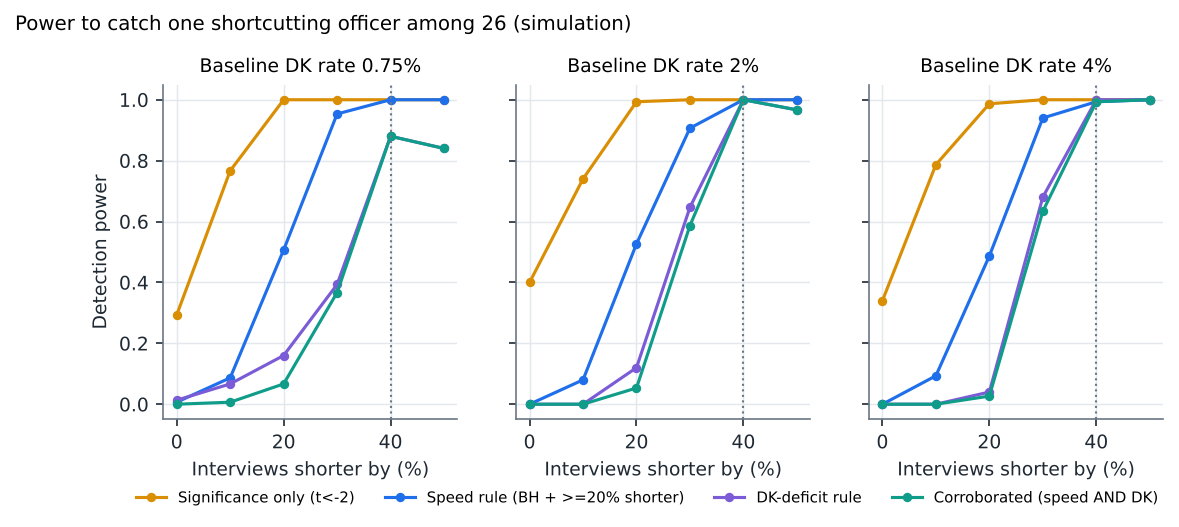
\includegraphics[width=\textwidth]{figures/fig03_power.png}\caption{Detection power by degree of shortening, for three baseline don't-know rates. \simd}\end{figure}
\begin{table}[H]\centering\footnotesize\setlength{\tabcolsep}{4pt}
\begin{tabular}{lrrrrrr}
\toprule
Shorter & Sig. pow. & Sig. FP & Speed pow. & Speed FP & Corr. pow. & Corr. FP \\
\midrule
0\% & 34 & 30.0 & 0 & 0.5 & 0 & 0.0 \\
10\% & 79 & 28.8 & 9 & 0.4 & 0 & 0.0 \\
20\% & 99 & 25.8 & 49 & 0.2 & 3 & 0.0 \\
30\% & 100 & 24.8 & 94 & 0.3 & 63 & 0.0 \\
40\% & 100 & 21.6 & 99 & 0.2 & 99 & 0.0 \\
50\% & 100 & 20.4 & 100 & 0.2 & 100 & 0.0 \\
\bottomrule
\end{tabular}\caption{Power (pow.) and false-positive rate (FP), \%, by rule: significance only, speed rule, and corroborated rule. Baseline don't-know rate 4\%. \simd}\end{table}
Four results stand out.
\begin{enumerate}
\item \textbf{Statistical significance alone is the wrong rule.} It flags 30\% of honest officers, because honest officers differ in pace and the test is sensitive to small, real differences. A 20\% effect-size floor with false-discovery control cuts false positives to 0.5\%; corroboration cuts them to 0.0\%.
\item \textbf{Power rises steeply with the size of the shortcut.} Speed-rule power is 9\% at 10\% shorter, 49\% at 20\%, 94\% at 30\% and 99\% at 40\%.
\item \textbf{The don't-know deficit is weak where it is rare.} At the real PAD2 rate (0.75\%) the corroborated rule catches 88\% of 40\% shortcutters (the speed rule alone: 100\%; the don't-know rule alone: 88\%). At 4\% it catches 99\%. Teams should not rely on don't-know deficits when the base rate is low.
\item \textbf{Daily testing inflates alarms.} Running the monitor 28 times at a fixed threshold produces a false speed flag on about 1.3 of 28 days; requiring the flag to persist two days cuts this to 0.9. Detection of a 40\%-shorter officer is not delayed much: the median is about 23 interviews (day 3; day 4 with persistence), set mostly by the 20-interview floor.
\end{enumerate}

\subsection{Case study: the enumerator who is 40\% faster with fewer ``don't knows''}\label{sec:case}
This is the scenario in the application question, and the simulation answers it directly. Figure~\ref{fig:tree} gives the decision procedure. In the planted case the speed rule and the don't-know rule both fire on day 4, which escalates the officer to Red and triggers a back-check within 48 hours. The distinction that matters is \emph{what corroborates the speed signal}. A fast officer with normal don't-know rates, normal path lengths and normal call times is amber: observe, compare with peers on the same questionnaire path, and sample a small back-check. A fast officer with fewer don't-knows, more skip-trigger answers, or timing that is impossible for the call volume is a back-check now.
\begin{figure}[H]\centering
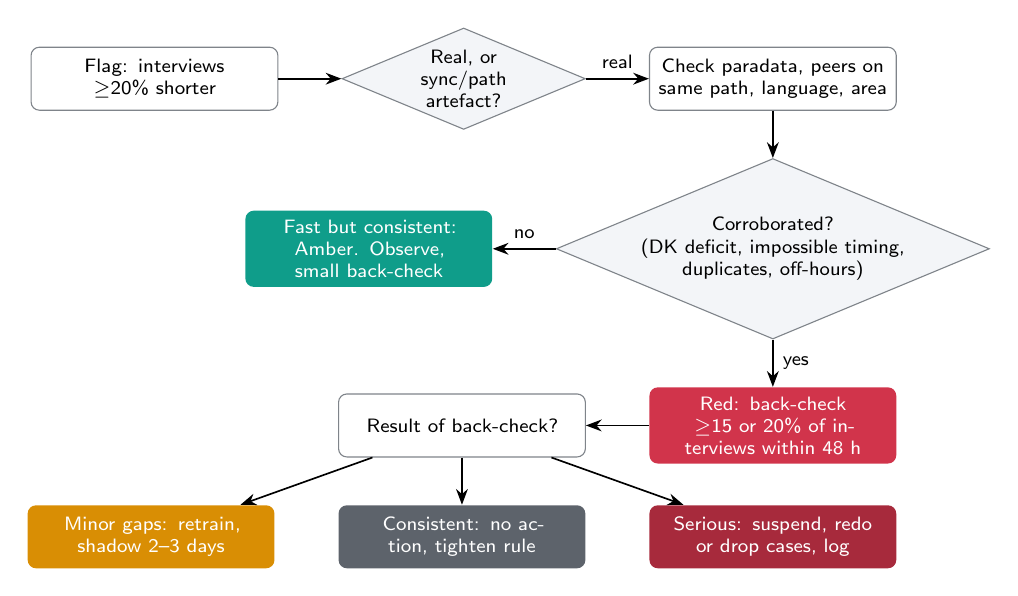
\begin{tikzpicture}[node distance=6mm and 8mm,font=\sffamily\scriptsize,d/.style={draw=ink!55,diamond,aspect=2.4,inner sep=1pt,align=center,fill=paper},b/.style={draw=ink!55,rounded corners=3pt,fill=white,align=center,minimum height=8mm,text width=29mm},o/.style={rounded corners=3pt,align=center,minimum height=8mm,text width=29mm,text=white},arr/.style={-{Stealth[length=2mm]},line width=0.6pt}]
\node[b](s){Flag: interviews $\ge$20\% shorter};\node[d,right=of s](v){Real, or\\sync/path\\artefact?};\node[b,right=of v](p){Check paradata, peers on same path, language, area};
\node[d,below=of p](c){Corroborated?\\(DK deficit, impossible timing,\\duplicates, off-hours)};
\node[o,fill=teal,left=of c](g){Fast but consistent: Amber. Observe, small back-check};\node[o,fill=red,below=of c](r){Red: back-check $\ge$15 or 20\% of interviews within 48 h};
\node[b,left=of r](t){Result of back-check?};
\node[o,fill=ink!70,below=6mm of t](x){Consistent: no action, tighten rule};\node[o,fill=amber,left=of x](y){Minor gaps: retrain, shadow 2--3 days};\node[o,fill=red!80!black,right=of x](z){Serious: suspend, redo or drop cases, log};
\draw[arr](s)--(v);\draw[arr](v)--node[above]{real}(p);\draw[arr](p)--(c);\draw[arr](c)--node[above]{no}(g);\draw[arr](c)--node[right]{yes}(r);\draw[arr](r)--(t);\draw[arr](t)--(x);\draw[arr](t)--(y);\draw[arr](t)--(z);
\end{tikzpicture}\caption{From flag to action. The SOP in the repository adds owners, timings and a log.}\label{fig:tree}\end{figure}

\section{What the programme did: experimental results}\label{sec:impact}
\subsection{Balance and attrition}
\real{} Randomisation balanced observables: the joint test that baseline covariates predict treatment gives $F=1.03$, $p=0.41$ in PAD2 ($F=0.61$, $p=0.72$ in PAD1); no single covariate differs at the 5\% level.
\begin{table}[H]\centering\small\setlength{\tabcolsep}{5pt}\begin{tabular}{lrrrr}
\toprule
Baseline variable & Control & Any SMS & Difference & p \\
\midrule
Age (years) & 42.10 & 41.44 & -0.680 & 0.062 \\
Female & 0.34 & 0.34 & +0.000 & 0.983 \\
Completed primary & 0.72 & 0.70 & -0.016 & 0.238 \\
Completed secondary & 0.13 & 0.13 & -0.000 & 0.970 \\
Prefers English & 0.36 & 0.35 & -0.013 & 0.349 \\
Mentions lime for acidity & 0.26 & 0.25 & -0.005 & 0.717 \\
Land size (acres) & 2.02 & 1.99 & -0.032 & 0.657 \\
Ever used lime & 0.09 & 0.09 & +0.005 & 0.526 \\
Used fertiliser last season & 0.87 & 0.89 & +0.013 & 0.169 \\
Lime recommended for soil & 0.77 & 0.76 & -0.005 & 0.407 \\
\bottomrule
\end{tabular}\caption{PAD2 baseline balance: any SMS versus control, with agrovet fixed effects. \real}\end{table}
Endline response was 84.1\% in control and 83.6\% among treated (difference -0.6 points, $p=0.61$); treatment-by-covariate interactions do not jointly predict response ($p=0.64$). Attrition is therefore unlikely to bias the estimates; Lee trimming bounds for lime use are narrow (4.8 to 5.5 points).

\subsection{Main effects}
Specification: outcome on a treatment indicator, gender, past lime use, age, land size, language and agrovet fixed effects, heteroskedasticity-robust standard errors. Holm adjustment covers the six outcomes.
\begin{table}[H]\centering\small\setlength{\tabcolsep}{4pt}\begin{tabular}{lrrrrr}
\toprule
Outcome & Control mean & ITT (pp) & SE (pp) & Holm p & N \\
\midrule
Heard of lime (survey) & 81.1\% & +5.51 & 1.24 & $<$0.001 & 4\,822 \\
Names lime as acidity remedy (survey) & 44.4\% & +10.22 & 1.56 & $<$0.001 & 4\,933 \\
Used lime, LR2017 (survey) & 17.5\% & +4.90 & 1.27 & $<$0.001 & 4\,933 \\
Used urea, LR2017 (survey) & 15.1\% & +3.32 & 1.19 & 0.016 & 4\,933 \\
Redeemed lime coupon (admin) & 10.7\% & +1.67 & 0.92 & 0.141 & 5\,890 \\
Redeemed fertiliser coupon (admin) & 8.7\% & -0.63 & 0.80 & 0.432 & 5\,890 \\
\bottomrule
\end{tabular}\caption{PAD2 intention-to-treat effects of any SMS versus control. \real}\end{table}
\begin{figure}[H]\centering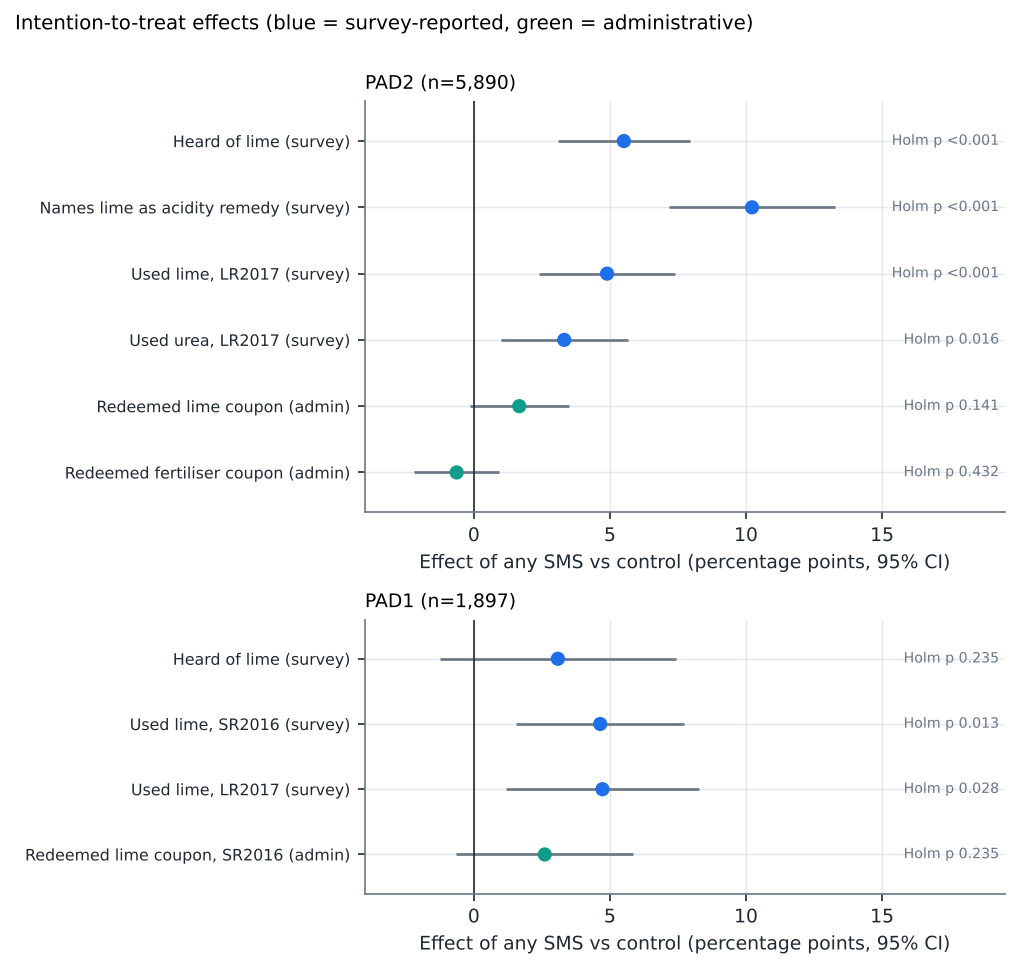
\includegraphics[width=0.74\textwidth]{figures/fig06_itt_forest.png}\caption{Effects with 95\% confidence intervals. Blue: survey-reported; green: administrative. \real}\end{figure}
Receiving SMS advice raised the share naming lime as a remedy for soil acidity by 10.2 points (control 44\%), and raised reported lime use by 4.9 points (95\% CI 2.4 to 7.4; control 18\%, a rise of about 28\%). Reported urea use rose by 3.3 points. All four survey effects survive Holm adjustment. PAD1 replicates the direction and size: reported lime use rose by 4.6 points in the first season and 4.7 points in the second (Holm $p=0.028$).
\begin{table}[H]\centering\small\setlength{\tabcolsep}{4pt}\begin{tabular}{lrrrrr}
\toprule
Outcome & Control mean & ITT (pp) & SE (pp) & Holm p & N \\
\midrule
Heard of lime (survey) & 77.7\% & +3.09 & 2.21 & 0.235 & 1\,471 \\
Used lime, SR2016 (survey) & 7.6\% & +4.64 & 1.58 & 0.013 & 1\,511 \\
Used lime, LR2017 (survey) & 11.2\% & +4.73 & 1.81 & 0.028 & 1\,511 \\
Redeemed lime coupon, SR2016 (admin) & 13.1\% & +2.61 & 1.66 & 0.235 & 1\,897 \\
\bottomrule
\end{tabular}\caption{PAD1 intention-to-treat effects. \real}\end{table}

\subsection{Survey versus administrative records}
The administrative lime effect is 1.7 points, about one third of the survey effect (ratio 2.9). The two are not the same construct, because farmers can buy lime without the coupon, and the administrative estimate is imprecise: with 5,890 farmers the minimum detectable effect is 2.6 points, larger than the estimate itself. What the comparison does show is that the survey figure cannot be taken at face value as a measure of adoption caused by the programme. If treated farmers over-report a behaviour they were advised to adopt, the survey effect (3.6 points is the MDE) is biased upward. I therefore present 4.9 points as an upper reading and the administrative figure as a lower one.

\subsection{Targeting}
Farmers were advised to use lime only where soil data called for it (77\% of the sample). The effect differs sharply by recommendation.
\begin{table}[H]\centering\small\setlength{\tabcolsep}{5pt}\begin{tabular}{lrrrr}
\toprule
Modifier & Group = 0 & Group = 1 & Interaction & p \\
\midrule
Lime recommended (soil pH) & -4.9 & +7.8 & +12.7 & $<$0.001 \\
Female & +5.7 & +3.2 & -2.5 & 0.357 \\
Used lime before baseline & +4.0 & +13.6 & +9.6 & 0.043 \\
\bottomrule
\end{tabular}\caption{PAD2 effect on reported lime use (pp) by baseline characteristic. Exploratory; no multiplicity adjustment. \real}\end{table}
\begin{figure}[H]\centering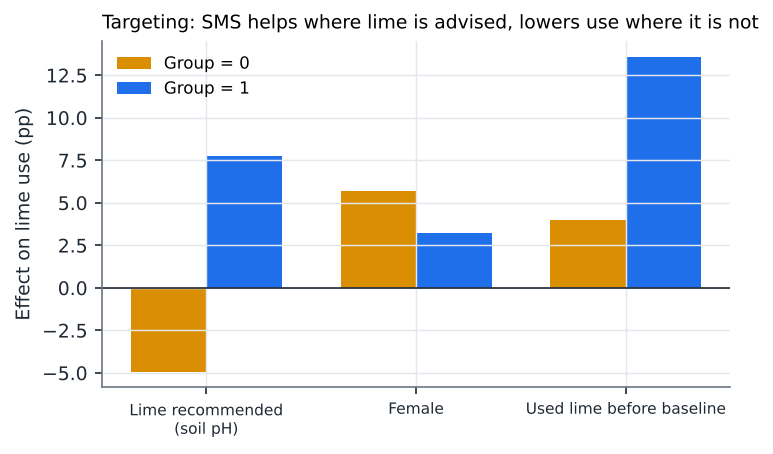
\includegraphics[width=0.55\textwidth]{figures/fig07_heterogeneity.png}\caption{SMS raises lime use where it is recommended and lowers it where it is not. \real}\end{figure}
Where lime was recommended, SMS raised lime use by 7.8 points; where it was not, it \emph{lowered} use by -4.9 points; the difference is 12.7 points ($p<0.001$). The administrative record agrees in sign ($2.9$ against $-2.3$ points; interaction $p=0.009$). Advice that tells farmers when \emph{not} to buy an input is rarely measured, and here it appears to work. This analysis was not pre-specified.

\subsection{Arms (secondary, with a caveat)}
\begin{table}[H]\centering\small\setlength{\tabcolsep}{5pt}\begin{tabular}{lrrrr}
\toprule
Outcome & SMS & SMS+Call offer & SMS+Call & p (arms equal) \\
\midrule
Names lime as acidity remedy (survey) & +9.7 & +9.3 & +11.7 & 0.379 \\
Used lime, LR2017 (survey) & +4.1 & +3.1 & +7.4 & 0.025 \\
Used urea, LR2017 (survey) & +3.3 & +1.5 & +5.2 & 0.060 \\
Redeemed lime coupon (admin) & +1.3 & +1.8 & +1.9 & 0.845 \\
\bottomrule
\end{tabular}\caption{PAD2 arm-level effects (pp). Arm labels follow the replication code's variable labels; see Section 2.4. \real}\end{table}
Arm differences are suggestive at best for lime use ($p=0.025$ for equality) and the ordering between \emph{SMS} and \emph{SMS+Call} would reverse if the two raw labels were swapped. I make no claim about whether calls add value.

\section{Does data quality change the conclusions?}\label{sec:robust}
\subsection{Officer effects}
\real{} Officers differ in the answers they record, even after adjustment. The intra-officer correlation is 4.0\% for ``heard of lime'' and 3.1\% for naming lime as a remedy, and 0.61\% and 0.57\% for lime and urea use (Table~\ref{tab:icc}). On a design with about 190 interviews per officer these produce large design effects, so a team that clusters errors on officer would see very wide intervals for knowledge outcomes.
\begin{table}[H]\centering\small\setlength{\tabcolsep}{5pt}\begin{tabular}{lrrr}
\toprule
Outcome & ICC (\%) & Design effect & p \\
\midrule
Heard of lime (survey) & 3.98 & 8.3 & $<$0.001 \\
Names lime as acidity remedy (survey) & 3.10 & 6.9 & $<$0.001 \\
Used lime, LR2017 (survey) & 0.61 & 2.1 & $<$0.001 \\
Used urea, LR2017 (survey) & 0.57 & 2.1 & 0.001 \\
\bottomrule
\end{tabular}\caption{Intra-officer correlation of PAD2 survey outcomes. \real}\label{tab:icc}\end{table}
Why does this not threaten the treatment effect? Because treatment is orthogonal to officer: officers' caseloads are balanced across arms (arm-by-officer $\chi^2$ $p=0.26$), so officer differences add noise to the estimate without biasing it.

\subsection{Four ways to treat officer quality}
\begin{table}[H]\centering\small\setlength{\tabcolsep}{5pt}\begin{tabular}{lrrrr}
\toprule
Specification & ITT (pp) & SE (pp) & p & N \\
\midrule
Baseline (all interviews) & 4.90 & 1.27 & $<$0.001 & 4\,933 \\
SE clustered by field officer & 4.90 & 1.45 & 0.002 & 4\,933 \\
+ field-officer fixed effects & 5.02 & 1.27 & $<$0.001 & 4\,933 \\
Drop Red-tier FOs & 5.12 & 1.35 & $<$0.001 & 4\,449 \\
Green-tier FOs only & 6.83 & 1.63 & $<$0.001 & 2\,990 \\
\bottomrule
\end{tabular}\caption{PAD2 effect on reported lime use under alternative treatments of officer quality. \real}\end{table}
\begin{figure}[H]\centering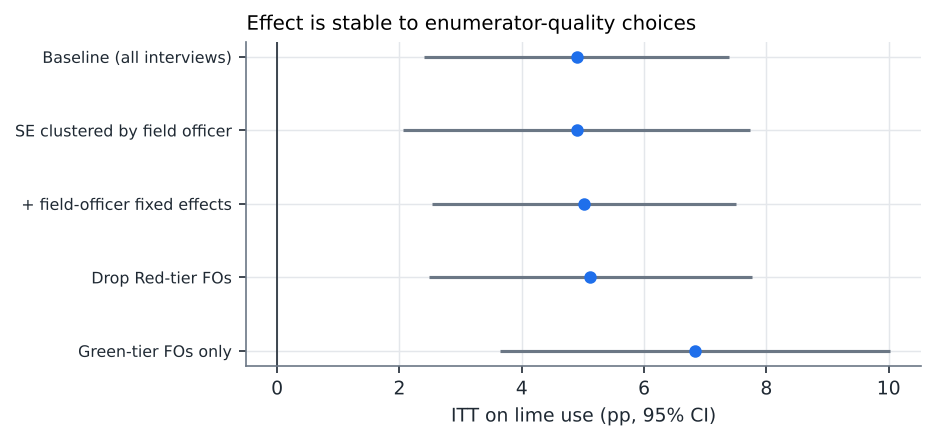
\includegraphics[width=0.58\textwidth]{figures/fig08_robustness.png}\caption{The estimate is stable. \real}\end{figure}
The effect is 4.9 points at baseline, 5.0 with officer fixed effects, and 5.1 after dropping the four red officers (4\,449 interviews). Clustering errors on officers widens the standard error from 1.3 to 1.4 points but leaves it clearly positive. Restricting to green officers gives 6.8 points on 2\,990 interviews, a larger but less precise estimate that is statistically compatible with the others.

\subsection{Do flagged officers report different outcomes?}
Across the 26 officers, the correlation between an officer's shortened-path effect and the officer's average (adjusted) reported lime use is 0.38 (permutation $p=0.057$). That is suggestive, not conclusive. Because path length depends on answers, a positive correlation is also what genuinely different caseloads would produce. It is another reason to verify by back-check and not to drop interviews on the basis of the flag alone.

\section{Recommendations: an operating procedure}\label{sec:recs}
\begin{enumerate}
\item \textbf{Program quality into the form.} Double ID entry, hard constraints with messages, one don't-know convention, paradata on by default, encryption key before the first call.
\item \textbf{Run the HFC daily; report by family.} One scorecard per officer, tiers fixed in advance, minimum 30 interviews before tiering, persistence rule for early days.
\item \textbf{Gate every rule on informativeness.} Disable checks whose base rate makes them meaningless (duplicate vectors in PAD2); keep skip-logic checks as regression tests.
\item \textbf{Never act on a single signal.} Fast alone is amber. Corroborated, or impossible timing, is a back-check within 48 hours.
\item \textbf{Calibrate with simulation.} Before fieldwork, plant problems in a copy of the instrument's expected data and measure power and false alarms. Do it again when thresholds change.
\item \textbf{Report quality next to results.} Show the estimate under officer fixed effects and without red officers, and show administrative outcomes where they exist.
\item \textbf{Record every decision.} Flag, evidence, action, outcome, in a log the PI can read.
\end{enumerate}

\section{Limitations and integrity notes}\label{sec:limits}
\begin{itemize}
\item \textbf{Paradata are simulated.} All timing results describe detector performance under stated assumptions (log-normal durations, don't-know rate 0.75--4\%, 20-interview floor). Real durations will be messier.
\item \textbf{Officer assignment is not randomised.} Differences are adjusted for arm, covariates and location only.
\item \textbf{Arm labels are ambiguous} in the replication files; the primary contrast avoids the problem.
\item \textbf{Method change disclosed.} A first pass with Welch tests flagged 6 of 25 PAD2 officers red; it was replaced by permutation inference, metric families and null calibration for statistical validity, before the numbers here were produced.
\item \textbf{Stata and XLSForm status.} The do-files were not executed and the form was validated structurally (no pyxform/ODK/SurveyCTO compiler was available). Run the comparison do-file and the 21-case test plan before relying on either.
\item \textbf{Heterogeneity analysis} is exploratory. \textbf{Survey effects} may be inflated by reporting bias.
\item Package installation from the Python index was blocked in the build environment, so regression and multiple-testing routines are implemented directly with NumPy and SciPy.
\end{itemize}

\appendix
\section{HFC rule reference}\label{app:hfc}
\small\setlength{\tabcolsep}{4pt}
\begin{tabular}{p{1.1cm}p{4.0cm}p{2.7cm}p{6cm}}\toprule ID & Check & Concerning & Note\\\midrule
H1 & Path length (items answered) & shorter than peers & Partly answer-driven; family ``shortcut''\\
H2 & Gate answered ``No'' & more than peers & Same family as H1\\
H3 & Don't-know share & fewer than peers & Weak when base rate $<1\%$\\
H4 & Straight-lining (6+ yes/no) & more than peers & Base rate about 1\%\\
H5 & Skip-logic violations (7 rules) & any & Zero in PAD1 and PAD2\\
H6 & Duplicate answer vectors & more than peers & Disabled if $>5\%$ duplicate by chance\\
H7 & Survey vs coupon discordance & more than peers & Purchase is not use; compare officers\\
H8 & Heaping on multiples of 5 & more than peers & PAD1 only; descriptive\\
R1--R6 & Speed, DK deficit, duplicates, off-hours, impossible timing, drift & see specification & Simulated paradata\\\bottomrule\end{tabular}
\normalsize

\section{Data-protection protocol (summary)}\label{app:dp}
Classify variables (direct identifiers, quasi-identifiers, analysis variables); minimise collection; encrypt at source with a key held offline by two custodians; keep the identifier crosswalk apart from analysis data; named, least-privilege access with periodic review; de-identify before sharing (remove identifiers, coarsen location, top-code, drop free text); approved encrypted transfer only; fixed retention and documented deletion; 24-hour incident reporting with remote wipe. The full protocol is in \texttt{docs/DATA\_PROTECTION\_PROTOCOL.md}. This repository ships no raw or identified data.

\section{Integrity checks run by the panel builder}
\small\setlength{\tabcolsep}{6pt}\begin{center}\begin{tabular}{l}
\toprule
Integrity check (all passed) \\
\midrule
PAD2 baseline: respid unique \\
PAD2 randomization: respid unique \\
PAD2 lime\_rec: respid unique \\
PAD2 endline: respid unique \\
PAD2 lime\_coupon: respid unique \\
PAD2 fert\_coupon: respid unique \\
PAD2 randomization covers baseline \\
PAD2 endline respondents all in baseline \\
PAD2 all arms mapped \\
PAD2 endline N matches raw \\
PAD2 responders have FO id \\
PAD2 treated share ~75\% \\
PAD2 outcomes binary \\
PAD1 baseline: respid unique \\
PAD1 treatment: respid unique \\
PAD1 endline: respid unique \\
PAD1 coupon: respid unique \\
PAD1 endline N matches raw \\
PAD1 responders have FO id \\
\bottomrule
\end{tabular}\end{center}\normalsize

\section{Reproducibility}
\begin{tabular}{p{4.2cm}p{10cm}}\toprule Path & Purpose\\\midrule
\texttt{python/01\_build\_panel.py} & Merge, harmonise, validate; writes panels and build log\\
\texttt{python/02\_hfc\_real.py} & HFC engine, permutation tests, tiering, null calibration\\
\texttt{python/03\_paradata\_simulation.py} & Planted problems, daily monitor, power, detection delay\\
\texttt{python/04\_impact.py} & Balance, attrition, ITT, Holm/BH, officer effects, robustness\\
\texttt{python/05\_figures.py}, \texttt{07\_key\_numbers.py} & Figures; single source of every headline number\\
\texttt{python/06\_build\_xlsform.py} & XLSForm build and structural validation\\
\texttt{python/08\_dashboard.py}, \texttt{09\_report.py} & Dashboard and this report (numbers read from outputs)\\
\texttt{stata/00\_master.do} \ldots\ \texttt{99\_compare\_python.do} & Stata mirror (unexecuted) and a parity assertion\\
\texttt{docs/} & HFC specification, data notes, back-check SOP, data protection, test plan\\\bottomrule\end{tabular}

Run \texttt{./run\_all.sh}. A single seed (20261101) governs every stochastic step. Raw data are obtained from openICPSR (project 186241); see \texttt{data/README.md}.

\section{Method details}\label{app:method}
\subsection{Permutation scoring of officers}
For each interview metric $m$ (path length, gate-``No'' count, don't-know share, straight-lining, duplicate flag, survey--coupon discordance) I residualise $y_{im}$ on arm, baseline covariates and location fixed effects, giving $\tilde y_{im}$. For officer $j$ with $n_j$ interviews the statistic is the standardised difference
\[ z_{jm}=\frac{\bar{\tilde y}_{jm}-\bar{\tilde y}_{m}}{\mathrm{sd}(\tilde y_m)} . \]
Officer labels are then permuted \emph{within location} $B=4{,}000$ times, which preserves each location's mix of officers and so respects the non-random assignment. The two-sided permutation $p$-value is $(1+\#\{|z^{*}_{jm}|\ge|z_{jm}|\})/(B+1)$. Benjamini--Hochberg q-values are computed across officers within each metric.

\subsection{Tiering}
An officer-metric is \emph{flagged amber} if $q\le0.10$ and $|z|\ge0.25$, \emph{red} if $q\le0.05$ and $|z|\ge0.25$; officers with fewer than 30 interviews are ``insufficient''. Metrics are collected into families (shortcut, don't-know, straight-line, logic, duplicate, administrative); an officer is \textbf{Red} if two families are red or three are flagged, \textbf{Amber} if any family is flagged, otherwise \textbf{Green}. Thresholds are fixed before looking at results and are the first thing to revisit after a pilot.

\subsection{Null calibration}
To check the whole procedure rather than a single test, officer labels are shuffled across the sample 300 times and the full tiering rule is rerun. The distribution of the number of flagged officers under shuffling is the benchmark in Figure~\ref{fig:null}.

\subsection{Treatment effects}
For outcome $y_i$ of farmer $i$ at agrovet $a$:
\[ y_{ia}=\alpha+\beta\,T_i+X_i'\gamma+\mu_a+\varepsilon_{ia}, \]
where $T_i$ indicates any SMS arm, $X_i$ is gender, past lime use, age, land size and language, and $\mu_a$ are agrovet fixed effects. Standard errors are HC1; officer-clustered standard errors use CR1. Holm adjustment covers the six outcomes. Lee bounds trim the group with higher response to the quantile that equalises response rates. Minimum detectable effects use $2.8\,\mathrm{SE}$ (80\% power, 5\% two-sided). Intra-officer correlation comes from one-way ANOVA with the unbalanced-cluster correction.

\section{Instrument test plan and Stata map}
The 21-case XLSForm test plan (\texttt{docs/XLSFORM\_TEST\_PLAN.csv}) covers: ID double entry mismatch and match; each skip pattern; the land-size and lime-area constraints with both valid and invalid values; don't-know propagation ($-99$ on land size must not block the lime-area check); mutually exclusive multi-select options; the implausible-lime-rate warning; the too-fast flag; the audit and duration fields; and encryption configuration. Each case lists inputs, expected behaviour and a pass/fail column to be completed on a SurveyCTO test server.

\begin{center}\small\setlength{\tabcolsep}{5pt}\begin{tabular}{p{4.3cm}p{9.7cm}}\toprule Stata file & Role\\\midrule
\texttt{00\_master.do} & Paths, globals, log, runs the sequence\\
\texttt{01\_clean\_pad2.do} & Merge, labels, derived outcomes, assertions\\
\texttt{02\_hfc\_enumerator.do} & Officer metrics and Welch comparisons (a simpler mirror of the permutation engine)\\
\texttt{03\_balance\_attrition.do} & Balance and attrition tables\\
\texttt{04\_itt.do} & ITT with agrovet fixed effects, Holm adjustment\\
\texttt{05\_fo\_effects.do} & Officer effects, ICC, robustness\\
\texttt{99\_compare\_python.do} & Reads Python outputs and asserts agreement within tolerance\\\bottomrule\end{tabular}\end{center}
The do-files use \texttt{assert} liberally and write logs. They have not been run here; the comparison do-file is the acceptance test.

\section{Questions this project is built to answer in a role like this}
\begin{itemize}
\item \textbf{How would you know a field officer is cutting corners?} Section~\ref{sec:audit}: adjusted peer comparison, permutation inference, corroboration across behaviours.
\item \textbf{What do you do when a check fires?} Section~\ref{sec:case} and the back-check SOP: verify, corroborate, back-check within 48 hours, record the outcome.
\item \textbf{How do you stop a check from crying wolf?} Section~\ref{sec:sim}: effect-size floors, false-discovery control, persistence, informativeness gates, simulation before fieldwork.
\item \textbf{Does it change the answer?} Section~\ref{sec:robust}: four treatments of officer quality, administrative outcomes, Lee bounds.
\item \textbf{Can someone else run it?} One command, one seed, outputs feeding every number in this report.
\end{itemize}
\end{document}
